\documentclass[11pt,a4paper]{article}

% ======== PAQUETES BÁSICOS ========
\usepackage[utf8]{inputenc}    % Acentos
\usepackage[T1]{fontenc}
\usepackage[spanish]{babel}    % Idioma español
\usepackage{amsmath, amssymb, amsfonts}  % Matemática
\usepackage{graphicx}          % Imágenes
\usepackage{physics}           % Derivadas, gradientes, etc.
\usepackage{siunitx}           % Unidades físicas (m, s, kg, etc.)
\usepackage{xcolor}            % Colores
\usepackage{geometry}          % Márgenes
\usepackage{fancyhdr}          % Encabezado/pie
\usepackage{hyperref}          % Enlaces
\usepackage{listings}          % Código fuente
\usepackage{caption}           % Subtítulos en código
\usepackage{tcolorbox}         % Cajas para resúmenes o ejemplos

% ======== CONFIGURACIÓN DE PÁGINA ========
\geometry{margin=2cm}
\pagestyle{fancy}
\fancyhf{}
\rhead{Apuntes de Física y Python}
\lhead{Israel Bravo — UdeC}
\cfoot{\thepage}

% ======== CONFIGURACIÓN DE CÓDIGO PYTHON ========
\definecolor{lightgray}{gray}{0.95}
\definecolor{darkgreen}{rgb}{0,0.5,0}
\lstset{
    language=Python,
    backgroundcolor=\color{lightgray},
    commentstyle=\color{darkgreen},
    keywordstyle=\color{blue}\bfseries,
    stringstyle=\color{red},
    basicstyle=\ttfamily\footnotesize,
    frame=single,
    numbers=left,
    numberstyle=\tiny\color{gray},
    breaklines=true,
    showstringspaces=false,
    tabsize=4
}

% ======== ESTILO DE CAJAS ========
\tcbset{
    colback=blue!5!white,
    colframe=blue!70!black,
    fonttitle=\bfseries,
    coltitle=black,
    boxrule=0.8pt,
    arc=3pt
}

% ======== INICIO DEL DOCUMENTO ========
\begin{document}

\begin{center}
    {\LARGE \textbf{Metodo de Euler/Runge-Kutta}}\\[4pt]
    {\large Universidad de Concepción — Israel Bravo}\\[10pt]
    \hrulefill
\end{center}

\section{Metodo de Euler}
Para empezar con el metodo de Euler tenemos que establecer la forma general de las ecuaciones que resolveremos con este metodo:

\begin{equation}
	\frac{du}{dt} = f(u,t)
\end{equation}

al encontrar cualquier funcion de este tipo, el metodo de euler nos dice que:

\begin{equation}
	u_{n+1}=f_n+f(u_n,t_n) \Delta t
\end{equation}

Podemos hacer lo siguiente en python para programar un metodo de resolver edos de la siguiente manera:

\begin{lstlisting}[caption={Programar el metodo de Euler}]
#Primero que nada, definimos el metodo de euler como

def euler(f, u, t): 
    u = np.copy(u)
    dt = t[1] - t[0]
    for n in range(len(t)-1): 
        u[n+1] = u[n] + f(u[n], t[n])*dt

    return u
\end{lstlisting}
Con esto definido ya podemos empezar a usar el metodo de euler de la siguiente manera, no sin antes ver cual es la ecuacion que representa el pendulo simple

\begin{equation}
\begin{cases}
\dot{\theta} = \omega, \\
\dot{\omega} = -\frac{g}{l} \sin\theta, \\
\theta(0) = \theta_0, \\
\omega(0) = \omega_0
\end{cases}
\end{equation}
con esta ecuacion dada, podemos definir la edo que resolveremos ahora:


\begin{lstlisting}[caption={Definamos la funcion y todos los parametros}]
#Importemos los modulos numpy y ademas programemos la edo que resolveremos:
import numpy as np
import matplotlib.pyplot as plt
#Definamos los parametros:
g = 9.81
l = 1.0
dt = 0.01
t = np.arange(0,N*dt,dt)
#Una vez hecho esto, tenemos que definir los valores iniciales:
u0 = np.array([omega,- (g/l) * np.sin(theta)])
#Una vez hecho esto, podemos empezar a usar la funcion de euler, y ademas graficarla
# Inicializamos la matriz para almacenar la solucion
# Cada fila es [theta, omega]
u = np.zeros((N, 2))
u[0] = u0


#Ejecutamos euler
u = euler(f, u, t)




\end{lstlisting}

Y si hacemos el grafico de la funcion, nos quedaria lo siguiente:

\begin{figure}[h]  % 'h' indica aquí, también puedes usar t (top), b (bottom), p (page)
    \centering
    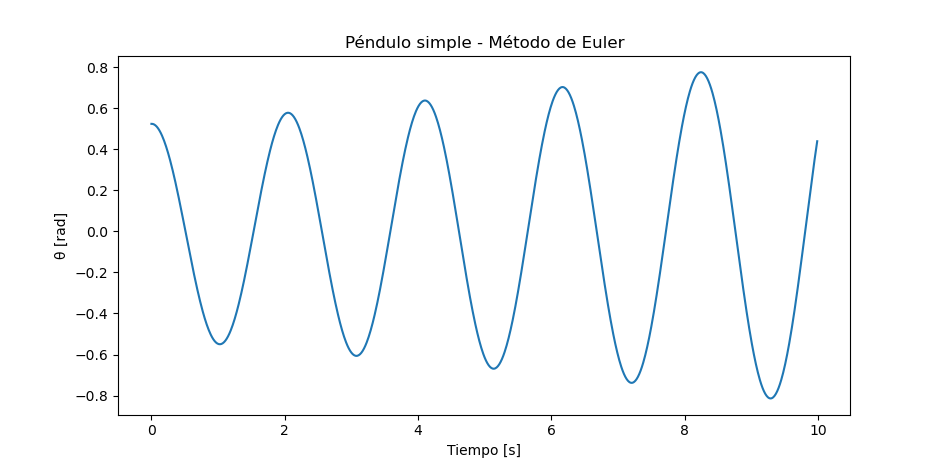
\includegraphics[width=0.9\textwidth]{img/Figure_1.png}  % ajustar ancho
    \caption{Pendulo simple}
    \label{fig:Pendulo_Simple}
\end{figure}

Se puede llegar a apreciar, el como esta funcion retrata al movimiento de este pendulo, de buena manera al principio, pero que segun van pasando los segundos cada vez va aumentando, esto se debe a que el metodo de euler es un metodo que no conserva la energia, y que va inyectando por asi decirlo energia y aumentandola. Esto se puede arreglar si disminuimos el valor de h, pero en si el metodo de euler es el peor metodo o de los peores para resolver edos, debido a este y otros problemas mas que conlleva usarlo.


\subsection{Pendulo doble}
Ahora resolveremos la ecuacion del pendulo pero esta vez sera doble. Esta ecuacion es un poco mas complicada y enrevesada de lo que es la Edo de un pendulo simple, se ve de la siguiente manera:


\begin{equation}
\begin{aligned}
\dot{\theta}_1 &= \omega_1, \\
\dot{\theta}_2 &= \omega_2, \\[0.5em]
\dot{\omega}_1 &=
\frac{
 -g (2m_1 + m_2)\sin\theta_1
 - m_2 g \sin(\theta_1 - 2\theta_2)
 - 2 \sin(\theta_1 - \theta_2) m_2
 \left[ \omega_2^2 l_2 + \omega_1^2 l_1 \cos(\theta_1 - \theta_2) \right]
}{
 l_1 \left[ 2m_1 + m_2 - m_2 \cos(2\theta_1 - 2\theta_2) \right]
}, \\[1em]
\dot{\omega}_2 &=
\frac{
 2 \sin(\theta_1 - \theta_2)
 \left[
  \omega_1^2 l_1 (m_1 + m_2)
  + g (m_1 + m_2)\cos\theta_1
  + \omega_2^2 l_2 m_2 \cos(\theta_1 - \theta_2)
 \right]
}{
 l_2 \left[ 2m_1 + m_2 - m_2 \cos(2\theta_1 - 2\theta_2) \right]
}.
\end{aligned}
\end{equation}




\begin{lstlisting}[caption={Edo pendulo doble}]
#Empecemos por definir la funcion que representa la edo 
import numpy as np
import matplotlib.pyplot
#Parametros fisicos
g = 9.81
m1, m2 = 1, 1
l1, l2 = 1, 1
#Definamos las condiciones iniciales ahora:
theta1_0 = np.pi/2
omega1_0 = 0
theta2_0 = np.pi/4
omega2_0 = 0
x0 = np.array([theta1_0,omega1_0,theta2_0,omega2_0])
\end{lstlisting}
\medskip

Definamos ahora la funcion vectorial $f(x,t)$




\end{document}
